\documentclass[tikz,border=12pt]{standalone}
% Shared visual language for standalone EMT block diagrams.
\usepackage{amsmath}
\usetikzlibrary{arrows.meta,backgrounds,calc,fit,positioning}

\tikzset{
    emt diagram/.style = {>={Stealth[length=2.4mm]}},
    line/.style        = {semithick, rounded corners=6pt},
    block/.style       = {draw, semithick, fill=white,
                          minimum height=1cm, minimum width=2.3cm},
    hblock/.style      = {block, minimum width=2.24cm, minimum height=1.3cm},
    vblock/.style      = {block, minimum width=1.3cm, minimum height=2.24cm},
    sum/.style         = {draw, semithick, fill=white, circle,
                          inner sep=2.6pt},
    signal/.style      = {circle, fill, inner sep=1.4pt,
                          label distance=3pt},
    sig/.style         = {font=\small},
    pm/.style          = {font=\scriptsize},
    wire jump/.style   = {line,
                          preaction={draw=white, line width=3pt,
                                     line cap=round}},
    enclosure/.style   = {draw, dashed, semithick, rounded corners=4pt},
    operator enclosure/.style = {enclosure, inner xsep=7mm, inner ysep=6mm}
}


\begin{document}
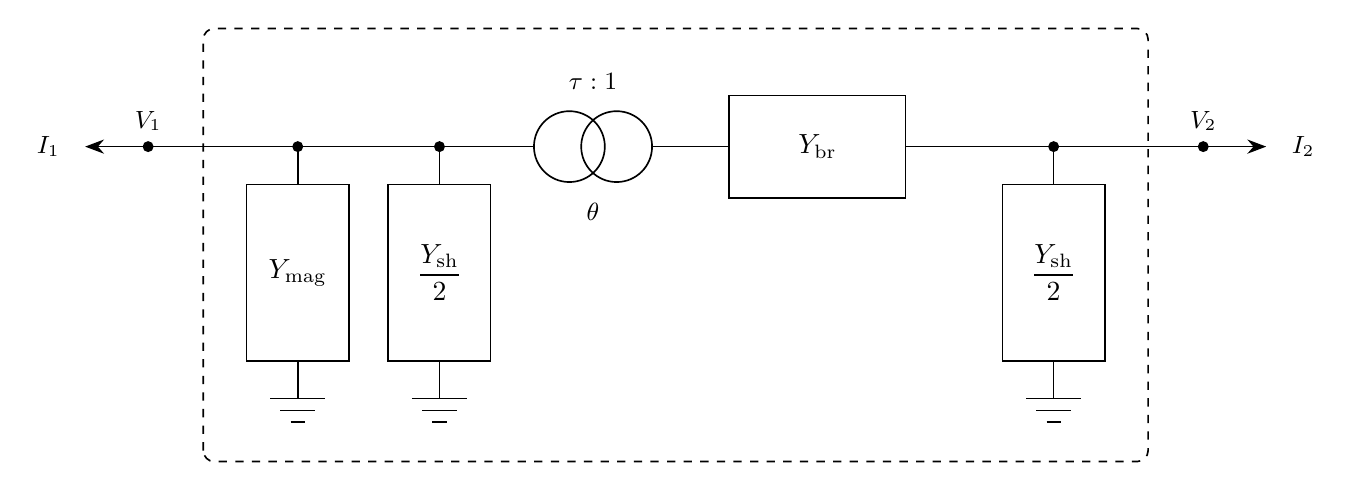
\begin{tikzpicture}[emt diagram]

% Branch network: shunts remain outside the bus-1 tap transformation.
\node[hblock] (series) at (1.8, 0) {$Y_\mathrm{br}$};
\node[vblock] (mag) at (-4.8, -1.6) {$Y_\mathrm{mag}$};
\node[vblock] (shunt1) at (-3.0, -1.6) {$\dfrac{Y_\mathrm{sh}}{2}$};
\node[vblock] (shunt2) at (4.8, -1.6) {$\dfrac{Y_\mathrm{sh}}{2}$};

% Single-line transformer symbol, with the tap on the bus-1 side.
\draw[semithick] (-1.35, 0) circle (0.45);
\draw[semithick] (-0.75, 0) circle (0.45);
\node[sig, anchor=south] at (-1.05, 0.6) {$\tau:1$};
\node[sig, anchor=north] at (-1.05, -0.6) {$\theta$};

\draw[line] (-0.3, 0) -- (series.west);

\foreach \shunt/\x in {mag/-4.8,shunt1/-3.0,shunt2/4.8} {
    \node[signal] at (\x, 0) {};
    \draw[line] (\x, 0) -- (\shunt.north);
    \draw[line] (\shunt.south) -- (\x, -3.2);
    \draw[semithick] (\x-0.35, -3.20) -- (\x+0.35, -3.20);
    \draw[semithick] (\x-0.22, -3.35) -- (\x+0.22, -3.35);
    \draw[semithick] (\x-0.09, -3.50) -- (\x+0.09, -3.50);
}

% Terminal voltages are bus-owned; current arrows point into the buses.
\draw[->, line] (-1.8, 0) -- (-7.5, 0);
\draw[->, line] (series.east) -- (7.5, 0);
\node[signal, label={[sig]above:$V_1$}] at (-6.7, 0) {};
\node[signal, label={[sig]above:$V_2$}] at (6.7, 0) {};
\node[sig, anchor=east] at (-7.7, 0) {$I_1$};
\node[sig, anchor=west] at (7.7, 0) {$I_2$};

% Model enclosure.
\draw[enclosure] (-6.0, -4.0) rectangle (6.0, 1.5);

\end{tikzpicture}
\end{document}
